\chapter{肺与气体交换}\label{ch:g7:lungs-and-gas-exchange}

在你的一生中，每分钟约有八升空气
流经两个你从未见过的器官。\Cref{ch:g4:breathing}
已勾勒了这条路径与交换；\cref{ch:g7:how-animals-breathe}
则将人体\omterm{def:g7:what-is-respiration:respiration}{呼吸}装置置于\omterm{def:g6:exploring-our-environment:components}{生物}界四大类群中加以比较。本章
补全这幅图景：通气装置、
以正式名称认识的\omterm{def:g7:lungs-and-gas-exchange:alveoli}{肺泡}、
气体交换的数量，以及烟雾对整套系统的危害。

\section{通气装置}

\begin{proposition}[空气如何进出]\label{prop:g7:lungs-and-gas-exchange:ventilation}
肺本身没有\omterm{def:g3:bones-and-muscles:muscle}{肌肉}；胸廓像风箱一样
带动肺的伸缩：
\begin{itemize}
  \item \omterm{def:g4:breathing:movements}{吸气}是\emph{做功}：肋间肌上提
        并使胸廓扩张，而
        \emph{膈肌}\index{膈肌}——宽阔的
        \omterm{def:g3:bones-and-muscles:muscle}{肌肉}底板，位于肺下方——向下压平；
        扩大的胸廓牵拉肺，
        空气流入以充满肺；
  \item 静止时的\omterm{def:g4:breathing:movements}{呼气}主要是\emph{放松}：
        \omterm{def:g3:bones-and-muscles:muscle}{肌肉}舒张，被拉伸的胸廓弹回，
        空气流出。（吹熄蜡烛时，\omterm{def:g3:bones-and-muscles:muscle}{肌肉}
        为胸廓的回弹添力。）
\end{itemize}
静止时每分钟约 $15$ 次
（见\cref{def:g4:breathing:movements}），无须主动调控，
（见\cref{rem:g5:brain-in-command:more}）——需要时便加深
并加快
（见\cref{prop:g7:organs-at-work:supply}）。
\end{proposition}
\admitted

\begin{example}[感受“风箱”]\label{ex:g7:lungs-and-gas-exchange:feel}
双手按住\omterm{def:g3:bones-and-muscles:skeleton}{肋骨}，深深\omterm{def:g4:breathing:movements}{吸气}：胸廓抬起并扩大，
在你的掌下（见\cref{ex:g4:breathing:watch}）。现在像狗一样
喘气：急促而浅的喘息几乎全靠
\omterm{prop:g7:lungs-and-gas-exchange:ventilation}{膈肌}完成。为完整起见，打嗝是
\omterm{prop:g7:lungs-and-gas-exchange:ventilation}{膈肌}抽搐般的误启动——风箱按自己的
节律失灵。
\end{example}

\section{肺泡与气体交换}

\begin{definition}[肺泡]\label{def:g7:lungs-and-gas-exchange:alveoli}
\cref{def:g4:breathing:organs}中所述的微小气囊，
即\emph{肺泡}\index{肺泡}：数以亿计
薄壁小泡，聚集在气道的最细末端，
每个小泡外都缠绕着细小的\omterm{def:g4:heart-and-blood:vessels}{血管}。它们的总表面积
相当于
\cref{rem:g4:breathing:sponge}中的半个网球场——这正是
\cref{prop:g7:how-animals-breathe:spec}所定的
“大、薄、湿”规格的人体版本。
\end{definition}

\begin{proposition}[气体交换的数量]\label{prop:g7:lungs-and-gas-exchange:numbers}
比较吸入与呼出的空气：
吸入的空气中，\omterm{def:g7:what-is-respiration:respiration}{氧气}约占 $21$\%，几乎不
含\omterm{def:g7:what-is-respiration:respiration}{二氧化碳}；呼出的空气中\omterm{def:g7:what-is-respiration:respiration}{氧气}降至约 $16$\%，
\omterm{def:g7:what-is-respiration:respiration}{二氧化碳}则升至约 $4$\%（此外还
温热湿润——
见\cref{ex:g4:breathing:mirror}）。两者之差即
气体交换：\omterm{def:g7:what-is-respiration:respiration}{氧气}穿过\omterm{def:g7:lungs-and-gas-exchange:alveoli}{肺泡}壁，
进入\omterm{prop:g4:journey-of-food:absorb}{血液}；\omterm{def:g7:what-is-respiration:respiration}{二氧化碳}则反向穿过
（见\cref{prop:g4:breathing:exchange}），
每分钟、每一天都在进行。
\end{proposition}
\admitted

\begin{omfigure}
\begin{tikzpicture}
  \node[anchor=south west, inner sep=0] (img) at (0,0)
    {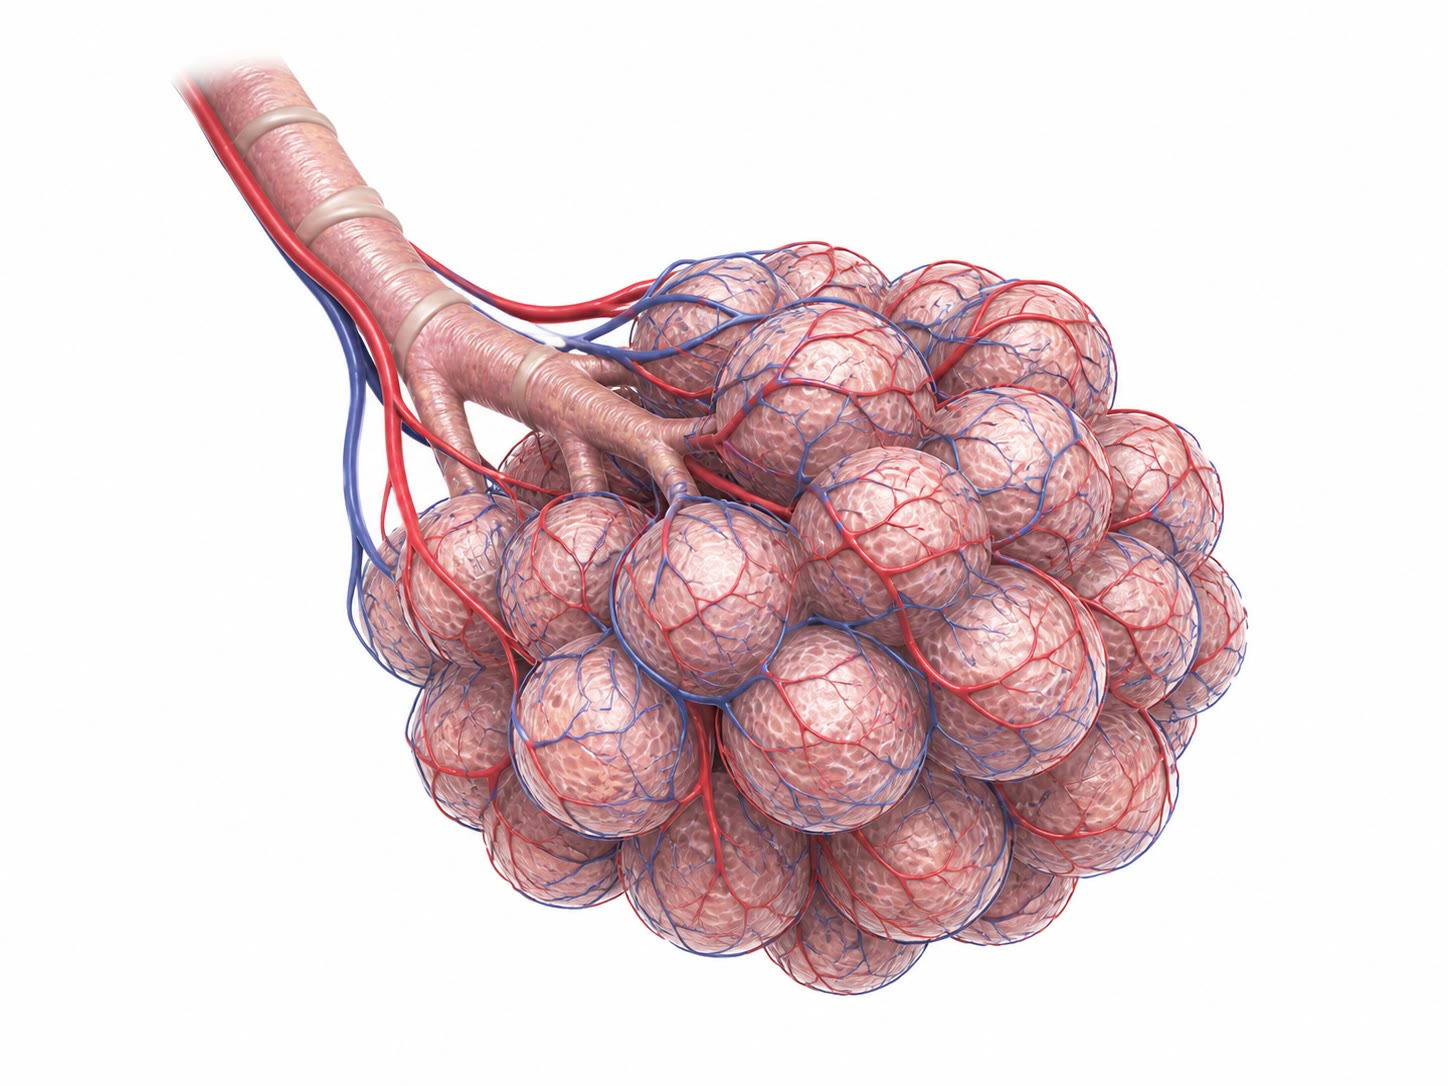
\includegraphics[width=0.6\linewidth]{images/book1/ai/fig-alveoli.jpg}};
  \begin{scope}[x={(img.south east)}, y={(img.north west)},
      every node/.style={font=\small}]
    \draw[omDef, thick] (0.24,0.83) -- (0.12,0.94)
      node[above] {最细气道};
    \draw[omThm, thick] (0.78,0.62) -- (0.90,0.80)
      node[above, align=center, omThm] {缠绕的 \\ 细血管};
    \draw[omMeth!60!black, thick] (0.46,0.34) -- (0.30,0.01)
      node[below, align=center, omMeth!60!black]
      {穿过每个小泡的薄壁：\\ 氧气入血，二氧化碳 \\
       反向回到空气中};
  \end{scope}
\end{tikzpicture}

{\small 数以亿计\omterm{def:g7:lungs-and-gas-exchange:alveoli}{肺泡}中的一簇：
薄壁小泡、缠绕的细\omterm{def:g4:heart-and-blood:vessels}{血管}，以及
双向交换这一核心作用。}
\end{omfigure}

\begin{example}[账目核对]\label{ex:g7:lungs-and-gas-exchange:accounting}
每分钟八升空气，每次吸入的\omterm{def:g7:what-is-respiration:respiration}{氧气}约有二十分之一
被留下：这一计算大致给出静止时身体的
耗氧量——而在费力活动时，\omterm{def:g7:what-is-respiration:respiration}{呼吸}增至三倍，
并加深，心跳也加快
（见\cref{prop:g7:organs-at-work:supply}），输送量
成倍增加，以匹配\omterm{def:g3:bones-and-muscles:muscle}{肌肉}的耗氧量。机器的
数字与身体的账目相互吻合；二者
是同一本账在两处记录。
\end{example}

\section{通气装置遭滥用：烟雾}

\begin{proposition}[烟雾对整套装置的影响]\label{prop:g7:lungs-and-gas-exchange:smoke}
烟草烟雾冲击本章所讲的每一层面
（\cref{prop:g5:healthy-choices:substances}已发出警告，
这里讲的是其工作原理）：
\begin{itemize}
  \item 焦油附着并刺激气道：
        清洁表面功能减弱，“吸烟者
        咳嗽”即是气道超负荷的“扫帚”；
  \item \omterm{def:g7:lungs-and-gas-exchange:alveoli}{肺泡}壁长期受刺激，
        逐渐崩解：小囊合并成数量更少、更大、更松弛的
        空间——\emph{表面积丧失}，连同
        气体交换随之受损（规格已被拆解）；
  \item 烟雾中的一种气体会占据\omterm{prop:g4:journey-of-food:absorb}{血液}中
        运输氧的结合位点，将\omterm{def:g7:what-is-respiration:respiration}{氧气}挤出其运输通道；
  \item 气道也随之变窄——每一次
        吸烟者每次\omterm{def:g7:what-is-respiration:respiration}{呼吸}，都是经由部分堵塞的
        风箱进行的。
\end{itemize}
这种损害缓慢、逐步累积，且仅
部分可逆：从未开始吸烟者的肺仍
完整保有半个网球场的表面积（见\cref{rem:g5:healthy-choices:never}）。
\end{proposition}
\admitted

\begin{example}[两次爬楼梯测试]\label{ex:g7:lungs-and-gas-exchange:stairs}
\cref{ch:g7:organs-at-work}中的三段楼梯，由两名年龄与训练习惯
相同的成年人攀登，其中一人是长期吸烟者：吸烟者
到达时已气喘吁吁、\omterm{prop:g4:heart-and-blood:pulse}{脉搏}飙升，
另一人只有冲刺时才达到相同的\omterm{prop:g4:heart-and-blood:pulse}{脉搏}。
表面积减少，结合位点被占，气道变窄——供应链通过被节流的进气口，
支付\cref{prop:g7:organs-at-work:bill}的账单。
体能测试能像任何扫描一样，
准确读出肺的过往。
\end{example}

\begin{method}[维护这台机器]\label{met:g7:lungs-and-gas-exchange:keep}
\Cref{met:g4:breathing:care}，
结合本章的理由加以升级：
\begin{enumerate}
  \item 不吸烟，无论是自己吸还是他人吸：
        已失去的表面积几乎无法\omterm{def:g7:organs-at-work:recovery}{恢复}；
  \item 为房间通风（见\cref{exo:g4:breathing:10}），
        运动时优先选择洁净的户外空气；
  \item 锻炼“风箱”：深\omterm{def:g7:what-is-respiration:respiration}{呼吸}的用力
        能锻炼\omterm{def:g7:what-is-respiration:respiration}{呼吸}肌，并使
        全部表面保持充分通气；
  \item 在寒冷多尘的\omterm{def:g6:exploring-our-environment:components}{环境}中用鼻子\omterm{def:g7:what-is-respiration:respiration}{呼吸}
        （见\cref{exo:g4:breathing:7}）——过滤器
        保护“扫帚”。
\end{enumerate}
\end{method}

\section{练习}

\begin{exercise}[$\star$]\label{exo:g7:lungs-and-gas-exchange:1}
将\omterm{def:g4:breathing:movements}{吸气}和\omterm{def:g4:breathing:movements}{呼气}描述为做功与释放：
分别涉及哪些\omterm{def:g3:bones-and-muscles:muscle}{肌肉}，发生了怎样的运动？
\end{exercise}

\begin{exercise}[$\star$]\label{exo:g7:lungs-and-gas-exchange:2}
\omterm{prop:g7:lungs-and-gas-exchange:ventilation}{膈肌}是什么？它位于何处？
\end{exercise}

\begin{exercise}[$\star$]\label{exo:g7:lungs-and-gas-exchange:3}
什么是\omterm{def:g7:lungs-and-gas-exchange:alveoli}{肺泡}——数量多少，壁是怎样构成的，
外面包裹着什么？
\end{exercise}

\begin{exercise}[$\star$]\label{exo:g7:lungs-and-gas-exchange:4}
请给出大致数值：吸入空气中的\omterm{def:g7:what-is-respiration:respiration}{氧气}、
呼出空气中的\omterm{def:g7:what-is-respiration:respiration}{氧气}，以及呼出空气中的\omterm{def:g7:what-is-respiration:respiration}{二氧化碳}。
这些数值之间的差值分别是多少？
\end{exercise}

\begin{exercise}[$\star$]\label{exo:g7:lungs-and-gas-exchange:5}
\omterm{def:g7:lungs-and-gas-exchange:alveoli}{肺泡}具备哪一项设计特点，
与本学年学过的另外哪两个器官共有这一特点？
\end{exercise}

\begin{exercise}[$\star$]\label{exo:g7:lungs-and-gas-exchange:6}
列出烟雾对这台“机器”发动的四种攻击中的三种。
\end{exercise}

\begin{exercise}[$\star\star$]\label{exo:g7:lungs-and-gas-exchange:7}
为什么\omterm{def:g4:breathing:movements}{吸气}需要做功，而静息时的\omterm{def:g4:breathing:movements}{呼气}
却不需要做功？向外的推力从何而来？
\end{exercise}

\begin{exercise}[$\star\star$]\label{exo:g7:lungs-and-gas-exchange:8}
请解释：失去的\omterm{def:g7:lungs-and-gas-exchange:alveoli}{肺泡}表面为什么无法
通过加快\omterm{def:g7:what-is-respiration:respiration}{呼吸}来补偿——气体交换中
缺少的是哪一个因素？
\end{exercise}

\begin{exercise}[$\star\star$]\label{exo:g7:lungs-and-gas-exchange:9}
请逐一解读\cref{ex:g7:lungs-and-gas-exchange:stairs}中的
两次爬楼梯测试，并将其逐一对应到
每一项攻击上。
\end{exercise}

\begin{exercise}[$\star\star$]\label{exo:g7:lungs-and-gas-exchange:10}
一名潜水员上浮时缓慢\omterm{def:g4:breathing:movements}{呼气}；一名小号演奏者
持续吹奏长而稳定的音符。
两者各自训练或使用的是
\cref{prop:g7:lungs-and-gas-exchange:ventilation}中的哪一环节？
\end{exercise}

\begin{exercise}[$\star\star$]\label{exo:g7:lungs-and-gas-exchange:11}
请将\cref{ex:g7:lungs-and-gas-exchange:accounting}
与\cref{prop:g7:organs-at-work:supply}加以对照：
哪三项调整能在用力时成倍增加供应，
它们各自分别对应哪一种限制因素？
\end{exercise}

\begin{exercise}[$\star\star\star$]\label{exo:g7:lungs-and-gas-exchange:12}
“肺是折叠进鞋盒里的、半个网球场大小的
边界，烟雾则是边界上缓慢燃烧的火。”
请结合本章的数字与机制，论证这两个
比喻的合理性。
\end{exercise}

\section{问题：呼吸机器档案}

\begin{problem}[{周末问题——一位工程师对人体
“风箱”的检查}]\label{pb:g7:lungs-and-gas-exchange:1}
一个工程课班级在纸面上“检查”人体的
\omterm{def:g7:what-is-respiration:respiration}{呼吸}机器：进气口、泵、交换表面、
运输连接与维护记录。

\medskip\noindent\textbf{第一部分——泵。}
\begin{enumerate}
  \item 画出泵的循环：两个时期、各自的驱动
        肌，以及在静息时哪一个时期
        消耗\omterm{prop:g3:balanced-diet:jobs}{能量}。
  \item 泵与被泵送器官自身的\omterm{def:g3:bones-and-muscles:muscle}{肌肉}没有
        接触——肺中也没有这类\omterm{def:g3:bones-and-muscles:muscle}{肌肉}。胸廓
        扩张究竟如何使空气流动？
  \item 给出泵的静息速率，以及它在用力时的
        两项调节
        （见\cref{prop:g7:organs-at-work:supply}）。
  \item 喘息、叹气、吹灭蜡烛：请把每一种
        归入循环机制中的相应位置。
\end{enumerate}

\medskip\noindent\textbf{第二部分——交换
表面}
\begin{enumerate}[resume]
  \item 说明表面的规格：名称、数量、
        壁、包裹方式及总面积。
  \item 对照
        \cref{prop:g7:how-animals-breathe:spec}中的规格，
        逐条核对。
  \item 吸入空气与呼出空气的成分相差
        本章所给的百分数。计算\omterm{def:g7:what-is-respiration:respiration}{氧气}的差值，
        以吸入空气中 $21$ 的百分数为基准，
——大约有多大比例的吸入\omterm{def:g7:what-is-respiration:respiration}{氧气}
        被保留下来？
  \item 呼出气体为什么必须保持温暖湿润——
        这是表面的哪种性质所付出的
        代价？
\end{enumerate}

\medskip\noindent\textbf{第三部分——维护
记录}
\begin{enumerate}[resume]
  \item 将烟雾的四种侵害归入：吸入、泵送、
        表面、运输。每项一行即可。
  \item 档案记录写道：“表面损失即资本损失。”
        请以咳嗽与感冒为例加以解释，
        它们相当于日常的小修小补。
  \item 写出维护计划——
        \cref{met:g7:lungs-and-gas-exchange:keep} ---
        以四条附理由的工程师指令形式给出。
  \item 作出检查结论：用一句话说明，
        在人体的泵与边界结构中，唯独这台机器
        为何有一半受主人的自主控制——
        这种控制用来做什么
        （如说话、歌唱，以及潜水员缓慢的\omterm{def:g4:breathing:movements}{呼气}）。
\end{enumerate}
\end{problem}
